\chapter{Towards model-based quality control}
\minitoc

% A few considerations:
% 1) The mathematical notation should be changed accordingly to Yves's suggestion in the paper
% 2) Some Figure could be replaced or improved. For instance, the Figure 4.7 should be replaced as well as the 4.15.


\section{Introduction}


In the manufacturing industry, product quality is an indicator for evaluating the production capacity of a company. Customers are increasingly demanding in terms of product quality and providing the customer with a product that complies with the specifications is absolutely essential in a market that is becoming more and more competitive. The best possible solution to deliver 100\% of compliant parts to the customer would be to inspect in details all parts produced. However, most companies cannot test every single product. There may simply be too high a volume or number of them to inspect at a reasonable cost or within a reasonable time frame. Or effective testing might result in the destruction of the product or render it unfit for sale in some way. Traditional quality inspection technology is the result of single variable statistical process control and sampling inspection.

One set of statistical tools for applying such a screening is acceptance sampling. Using such tools enables decision makers to determine what action to take on a batch of products. Decisions based on frequency testing, rather than on 100\% inspection, are more expedient and cost effective but it cannot guarantee the conformity of all parts of the population from which the sample was drawn~\citep{fuchs1998multivariate}.

In this chapter, we propose a new approach to perform a real-time, non-destructive quality control to measure thicknesses of blow-molded parts. The proposed approach makes use of deep learning data-driven methods to leverage the thermal inertia of the manufactured plastic part, captured through the use of thermal imaging, to infer the thicknesses of the part surface without any direct measurement. Compared to traditional quality inspection approaches, which aim to detect visual defects of manufactured products, our approach leverages thermal information to perform a non-visual quality control. 
%
The first experimental results on real industrial data are very promising and demonstrate that the proposed methods could achieve satisfactory performance for industrial usage.

\section{Towards data-driven quality control}

In this section, we extend the concept that was presented in Chapter \ref{From Corrective to Predictive Process Control} in order to develop a general framework for inferring the quality of a manufactured part without directly measuring it. One more time, we will take advantage of the ability of machine learning to learn the transfer function from some input data to the product quality. The trained model could then be applied to enhance the manufacturing quality control by providing a quality status to the part.

Historically, in the manufacturing industry, and in particular in the research framework that have been studied during this PhD study, the real quality control is a time-consuming operation that requires several minutes of work and that cannot be done online for each part. As a consequence, the only method that fits these production constraints is the \textit{Acceptance sampling} method. One part per \textit{X} parts produced is physically measured and the quality of the entire production batch is determined by the result obtained from the measurement on the individual sample. Figure \ref{fig:statistical_quality_control} outlines the functioning of acceptance sampling. 

\begin{figure}
\centering
\includegraphics[scale=0.50]{images/chapter_4/statistical_quality_control.png}
\caption{Statistical quality control}
\label{fig:statistical_quality_control}
\end{figure}

Although this method is widely applied in the manufacturing industry and it is globally accepted, it presents two major drawbacks:
\begin{enumerate}
    \item The acceptance sampling method is able to track deviations in product quality, but it is not able to provide 100\% quality inspection. As a result, it may happen that one or multiples non-compliant parts are produced, as a response to a temporary malfunction in the production process, and these parts may not be detected. This may result in one or multiple non-compliant parts being sent to the customer.
    \item The second drawback of Acceptance Sampling is the delay in detecting a process deviation. If product quality starts to deviate, the manufacturer has to wait for the next quality control to identify the problem and to be able to act on the process to correct it. Moreover, the parts produced in this time frame are potentially non-compliant and extra time-consuming quality control may be required to establish whether or not the parts can be sent to the customer.
\end{enumerate}

Another problem to consider, is the one related to the destruction of the pieces being measured. In fact, some quality measurements involve the destruction of the part or some modifications that make it unsuitable for sale to the customer. For instance, advanced quality control for assessing the material distribution of each thickness layer of a blow-molded part requires the cutting of the piece in small samples, subsequently analyzed in the laboratory. Even if these tests are necessary and important to certify the conformity of the part, it constitutes a source of waste for the manufacturer, increasing the number of PPM (parts per million) defects. 

In order to improve the quality control of the parts, we propose to perform a comprehensive quality control using a machine learning based approach. The idea is to infer the quality status of each part produced through the use of a machine learning algorithm. Unlike in Chapter 3, we are not bound to use the process data as a predictor for our model, because we are only interested in providing a status to a manufactured part and we are not directly concerned by the production process. New sensors or cameras may be installed to recover new sources of data ``close'' to the final product.

In the context of this PhD study, the approach of inferring the quality of a part using a trained machine learning algorithm is called \textit{data driven model-based quality control}.
The benefits that this approach can bring to quality control throughout the manufacturing industry are manifold. First, it ensures a 100\% quality control on all parts produced which enable for a fast reaction to quality non-conformities (Figure \ref{fig:model_quality_control} on the left side). In fact, by ``virtually'' measuring each part, we are able to eventually discard parts for which the model has provided a ``Not-OK'' result, or request the quality team to carry out more in-depth tests. Model-based quality measurement may be effectively used to detect those parts that turn out to be, from a statistical point of view, outliers. In this way, instead of randomly sampling the parts to be measured by the quality operators, the model is able to suggest the parts that seem to be interesting.
By discarding all non-compliant parts, this approach indirectly reduces product recalls and thus the whole series of requests to return, exchange or replace a product that has been found to be defective, and which could impair performance, harm consumers or cause legal problems for producers.

\begin{landscape}
\begin{figure}
\centering
\includegraphics[scale=0.50]{images/chapter_4/data_driven_model.png}
\caption{Data-driven model-based quality control}
\label{fig:model_quality_control}
\end{figure}
\end{landscape}

If the trained model is sufficiently robust and accurate at predicting the quality status of a part, a second stage would be to reduce the real quality controls which destroy the parts or makes them unusable (Figure \ref{fig:model_quality_control} on the right side). In such a case, not only the model-based control would be able to provide a thorough quality control, but it would also be able to reduce the quality PPM which account for an overall better production performance. Of course, real part measurements cannot be completely replaced by model-based measurements. In fact, real measurements are the primary data source for training the data-driven model. 

\section{Thickness inference using thermal imaging}

\subsection{Context and background} \label{Context and background}

In Blow-molded parts the material distribution all over the part surface plays a key role in ensuring that the finished product meets customer specifications. The thickness of the tank over the whole surface must be enough to ensure the robustness of the part and therefore its safety, while avoiding an excessive and unnecessary weight of the finished product. Measuring the thickness of a blow-molded part over its entire surface is trivial because most of the blow-molded parts are hollow, which limits how the thickness can be measured. Traditional methods to measure the thickness of hollow parts involve the use of ultrasonic measuring instruments that provide satisfactory results while avoiding the destruction of parts. The main idea of \textit{Ultrasonic Thickness Measurement} (UTM) is to measure the time needed for the ultrasonic wave to traverse the material. Some of the advantages of UTM over other nondestructive methods are:
\begin{itemize}
    \item the possibility to measure parts with just one accessible surface,
    \item no need for laboratory conditions,
    \item  its high sensitivity and accuracy.
\end{itemize}
 
Although these methods are extremely high-performance for sample quality control, they present a major drawback: they cannot be used for online measurement. The measurement of a large number of points, which is necessary to estimate the distribution of the material over the entire surface, is time-consuming and cannot be applied online in production. Hence, the quality control of the thickness can only be carried using a sampling approach. Recently, new technologies involving the use of terahertz waves have been developed to accurately measure the thickness of materials without any contact with the material itself. These methods have proven to be extremely powerful for measuring the thickness of automobile paint \citep{su2014terahertz,krimi2016highly}, or pharmaceutical tablets \citep{may2011terahertz}. Of all the methods found in the literature, terahertz-based systems seem to be the only ones that can be used to perform real-time thickness measurement, but in order to use it in real-time, the measurement sensor must be installed on a robot, or collaborative robot, which can significantly affect the price of the complete measurement solution.

Another well-known technique for measuring thickness of parts is \textit{Computed Tomography} (CT). Typical areas of use for CT in industry are in the detection of flaws such as voids and cracks, and particle analysis in materials. In metrology, CT allows measurements of the external as well as the internal geometry of complex parts. As stated by \citet{de2014industrial}, CT is particularly suitable to investigate molded polymer parts, thanks to the good penetrability of X-rays in these materials. Even if CT-based techniques are extremely powerful, they require laboratory conditions and  do not lend themselves well to real-time thickness control. Moreover, this equipment may be very expensive, questioning its profitability.
%
Eddy current testing, widely applied for the non-destructive thickness measurement of metallic parts \citep{cheng2017thickness,mao2016thickness,wang2015noncontact,yin2007thickness}  is also non-destructive, but cannot be used as polymers composing the blow-molded part are not conductive.

\textit{Thermal Imaging}, a non-contact technology capable of measuring large surfaces in a single shot, has been applied to different kinds of thickness prediction methods in the last decades \citep{sun2003method,sun2006analysis,choi2008quantitative,benitez2008definition,zeng2012absolute,li2018thickness,he2013eddy}. Among the most widely used thermal imaging approaches we can mention: \textit{Pulsed thermography} in which a brief controlled thermal stimulation pulse is applied on the tested piece, \textit{Step heating thermography} in which a continuous, uniform heat flow is applied for a long period, and \textit{Lockin thermography} in which a periodic heat input is used. The main idea behind all these approaches is to transfer energy to the test piece and to monitor its surface temperature evolution over time. In flash thermal imaging, for example, some flash lamps provide the thermal impulse, and the infrared camera monitors the surface-temperature decay on the heated surface. On the other hand, step-heating thermal imaging is using a long pulse of low intensity heat stimulation. Unlike pulsed thermal imaging, step-heating technology monitors the temperature raise over time while the heat energy is transferred to the test piece.
The approach of monitoring the surface-temperature may also be applied without actively providing heat to the test part, especially for parts that are still hot after the manufacturing process. This is definitely the case of blow-molded parts. Even if the part surface is cooled inside the molds during the blowing process, thicker blow-molded products still have high temperatures and it takes several minutes for the work-piece to reach the temperature of the environment in which it is cooled.

\subsection{Motivation} \label{Motivation}

Our work is motivated by the empirical observation of the cooling of blow-molded parts in the first minutes after blowing. Areas of the parts have different cooling behaviours depending on their thickness. 

Areas with smaller thicknesses cool down faster than those with larger thicknesses. For the thicker zones, the surface temperature even starts to increase before decreasing (Figure~\ref{fig:temperature_cooling}).
%
\begin{figure}
\centering
\includegraphics[scale=0.55]{images/chapter_4/cooling.eps}
\caption{Surface temperature cooling profiles at the thinnest (left) and thickest (right) areas of the blow-molded part}
\label{fig:temperature_cooling}
\end{figure}
%
This phenomenon is due to the release of energy from the innermost plastic layer that has not be in direct contact with the mold surfaces.
As suggested by the literature presented in Section \ref{Context and background}, this surface temperature decay, easily measured by thermal imaging, could be leveraged to infer the thickness of the part.  
In particular, we make two assumptions:
\begin{itemize}
   \item The cooling conditions of the environment where the part is monitored are the same for all parts produced. Therefore, we consider that the variations of the temperature of the production area are negligible.
   \item The physical and chemical properties of the material are assumed to be constant over the entire surface of the part. In particular, the thermal and infrared transmittances of the material should be approximately constant.
\end{itemize}

Based on these assumptions, we designed two data-driven methods to model the relationship between the surface temperature variations of critical areas of the part and the corresponding thickness values. The first approach, by one-dimensional time series, exploits the cooling dynamics, one point of the part at a time, whereas the second method processes the part globally, taking into account unity of part (points belonging to the same part are processed simultaneously) and spatial information (points are positioned on the part surface).

\subsection{Proposed methods}

In this section, we present new approaches to predict the thickness of blow-molded parts. We propose a non-intrusive real-time thickness inference exploiting the variations of surface temperatures over time on different areas of the blow-molded part. 
Unlike traditional thickness quality control methods, our system is able to predict thickness values at critical points of the part within minutes, allowing real-time operation.

Three different approaches to model the temperature-thickness relationship are proposed:
%
\begin{itemize}
    \item \textit{Functional approach}: The Functional approach involves the use of a parametric function to approximate the pixel-wise temperature surface decay. The function parameters, retrieved through the use of a curve fitting approach, may then be used as input features for a machine learning regressor.
    \item \textit{Temporal approach}: The Temporal approach, as the Functional one, takes advantage of the pixel-wise temperature decay. Instead of compressing the information through the use of a parametric function, the temporal approach leverages the ability of deep learning to extract meaningful features from raw signals.
    \item \textit{Spatial-Temporal approach}: The Spatial-Temporal approach leverages not only the temporal temperature information, but also the spatial one. Instead of extracting the temperature time series for each critical point of the blow-molded parts we can design an \textit{end-to-end} deep learning architecture able to directly handle the input thermal video. In such a way, we should be able to take into consideration not only the surface-temperature evolution of a point but also its position on the spatial dimension. 
\end{itemize}
%
These three approaches are presented in more detail below.

\subsubsection{Functional approach} \label{Functional approach}

The first approach consists of three phases: time series extraction, time series approximation by parametric curve fitting and thickness prediction using the parameters of the approximated temperature surface decay.

\paragraph{Time series extraction:} 

The time series extraction phase aims to process the input thermal video in order to retrieve the temperature time series of a limited number of critical points, for which the thickness value is known. These time series constitute the input data of our data-driven model.
Given $n$ critical points of each part, for which the thickness values are known, and given its thermal video $X^i$, we are interested in extracting the time series $ts^{i}_{(x_j, y_j)}$ where $j \in [1,n]$. For a set of $m$ input thermal video, this first phase produce a dataset
\begin{equation}
    D = \{(ts^{i}_{(x_j, y_j)}, y^{i}_{(x_j, y_j)});i \in [1, m]; j \in [1, n]\},
\end{equation}
composed of $n\times m$ collection pairs $(ts^{i}_{(x_j, y_j)}, y^{i}_{(x_j, y_j)})$ where $ts^{i}_{(x_j, y_j)}$ is the $j$-th time series extracted from the thermal video $i$ and $y^{i}_{(x_j, y_j)}$ is the corresponding thickness value. 

\paragraph{Time series approximation:}

In order to reduce the number of input features we made to choice to approximate the surface-temperature decay time series through the use of parametric function. Approximating the time series with a parametric function would allow to compress the temporal information in a limited number of new features, corresponding to the parameters of the function. Temperature-surface time series have a fairly simple shape to approximate (Figure \ref{fig:temperature_cooling}). The predominantly parabolic shape of the time series lends itself well to be approximated with a quite simple function with a few parameters. We compared the following three parametric models in order to find the one that best fits our time series:
\begin{itemize}
    \item Power Law: $y=ax^b$
    \item Polynomial (2° degree): $y=ax^2+bx+c$
    \item Logarithmic: $y=a+b\log(x)$
\end{itemize}

In such a way, the different cooling behaviour, observable in different areas of the part could be expressed through a limited number of new parameters (Figure \ref{fig:parametric_approximation}. Moreover, the functional approximation smooths the time signal, thereby reducing the measurement noise. The new features may be then used as the input data for a regression model. Mathematically speaking, the time series approximation produces a new dataset,
%
\begin{equation*}
    D = \{(z^{i}_{(x_j, y_j)}, y^{i}_{(x_j, y_j)});i \in [1, m]; j \in [1, n]\}
    \enspace,
\end{equation*}
%
composed of $n\times m$ collection pairs $(z^{i}_{(x_j, y_j)}, y^{i}_{(x_j, y_j)})$ where $z^{i}_{(x_j, y_j)}$ is the $j$-th set of parameters obtained by fitting the parametric function. 

\begin{figure}
\centering
\includegraphics[scale=0.9]{images/chapter_4/Parametric approximation (Polynomial).png}
\caption{Parametric approximation}
\label{fig:parametric_approximation}
\end{figure}

\paragraph{Time series regression:}
Parametric models such as \textit{Lasso Regression} (\ref{Parametric models}), or Decision-Tree based methods such as \textit{random forest} (\ref{Tree-based methods}) or even \textit{Support Vector Machine} (\ref{Support Vector Machines}) methods may than be applied to try to predict the thickness value of a given area based on the parametric features computed through the functional fitting of the surface-temperature time series. The role of the machine learning model is to learn the transfer function $\hat{f}$ which satisfies the following equation:

\begin{equation}
    y^{i}_{(x_j,y_j)} = \hat{f}(z^{i}_{(x_j, y_j)}; i \in \{1, \ldots,n\}; j \in \{1, \ldots,K\}) + \epsilon.
\end{equation} 

\subsubsection{Temporal approach}

The proposed method consists of two phases: extraction of the time series and thickness value regression through a Recurrent Neural Network based architecture (Figure \ref{fig:temporal_approach}). The time series extraction is carried out exactly in the same way as for the Functional approach (compare section \ref{Functional approach}).  

\begin{figure}
\centering
\includegraphics[scale=0.4]{images/chapter_4/temporal_approach.eps}
\caption{Temporal approach}
\label{fig:temporal_approach}
\end{figure}

\paragraph{Time series regression:}

Given the extracted time series and the corresponding thickness values, our problem could be formulated as a supervised machine learning problem, in particular, as a univariate time series regression problem. With univariate time series regression we mean the task of predicting the real number value of the dependent variable, the thickness, given a single dependent variable corresponding to a sequence of discrete-time data. 
Mathematically speaking, we look for the function $\hat{f}$ so that
\begin{equation}
    y^{i}_{(x_j,y_j)} = \hat{f}(ts^{i}_{(x_j, y_j)}; i \in [1, m]; j \in [1, n]) + \epsilon,
\end{equation} 
Since we are dealing with data where the temporal information plays a key role, according to our assumptions, in discriminating the thickness, we made the choice to use an approach based on recurrent neural network. 

\begin{figure}
\centering
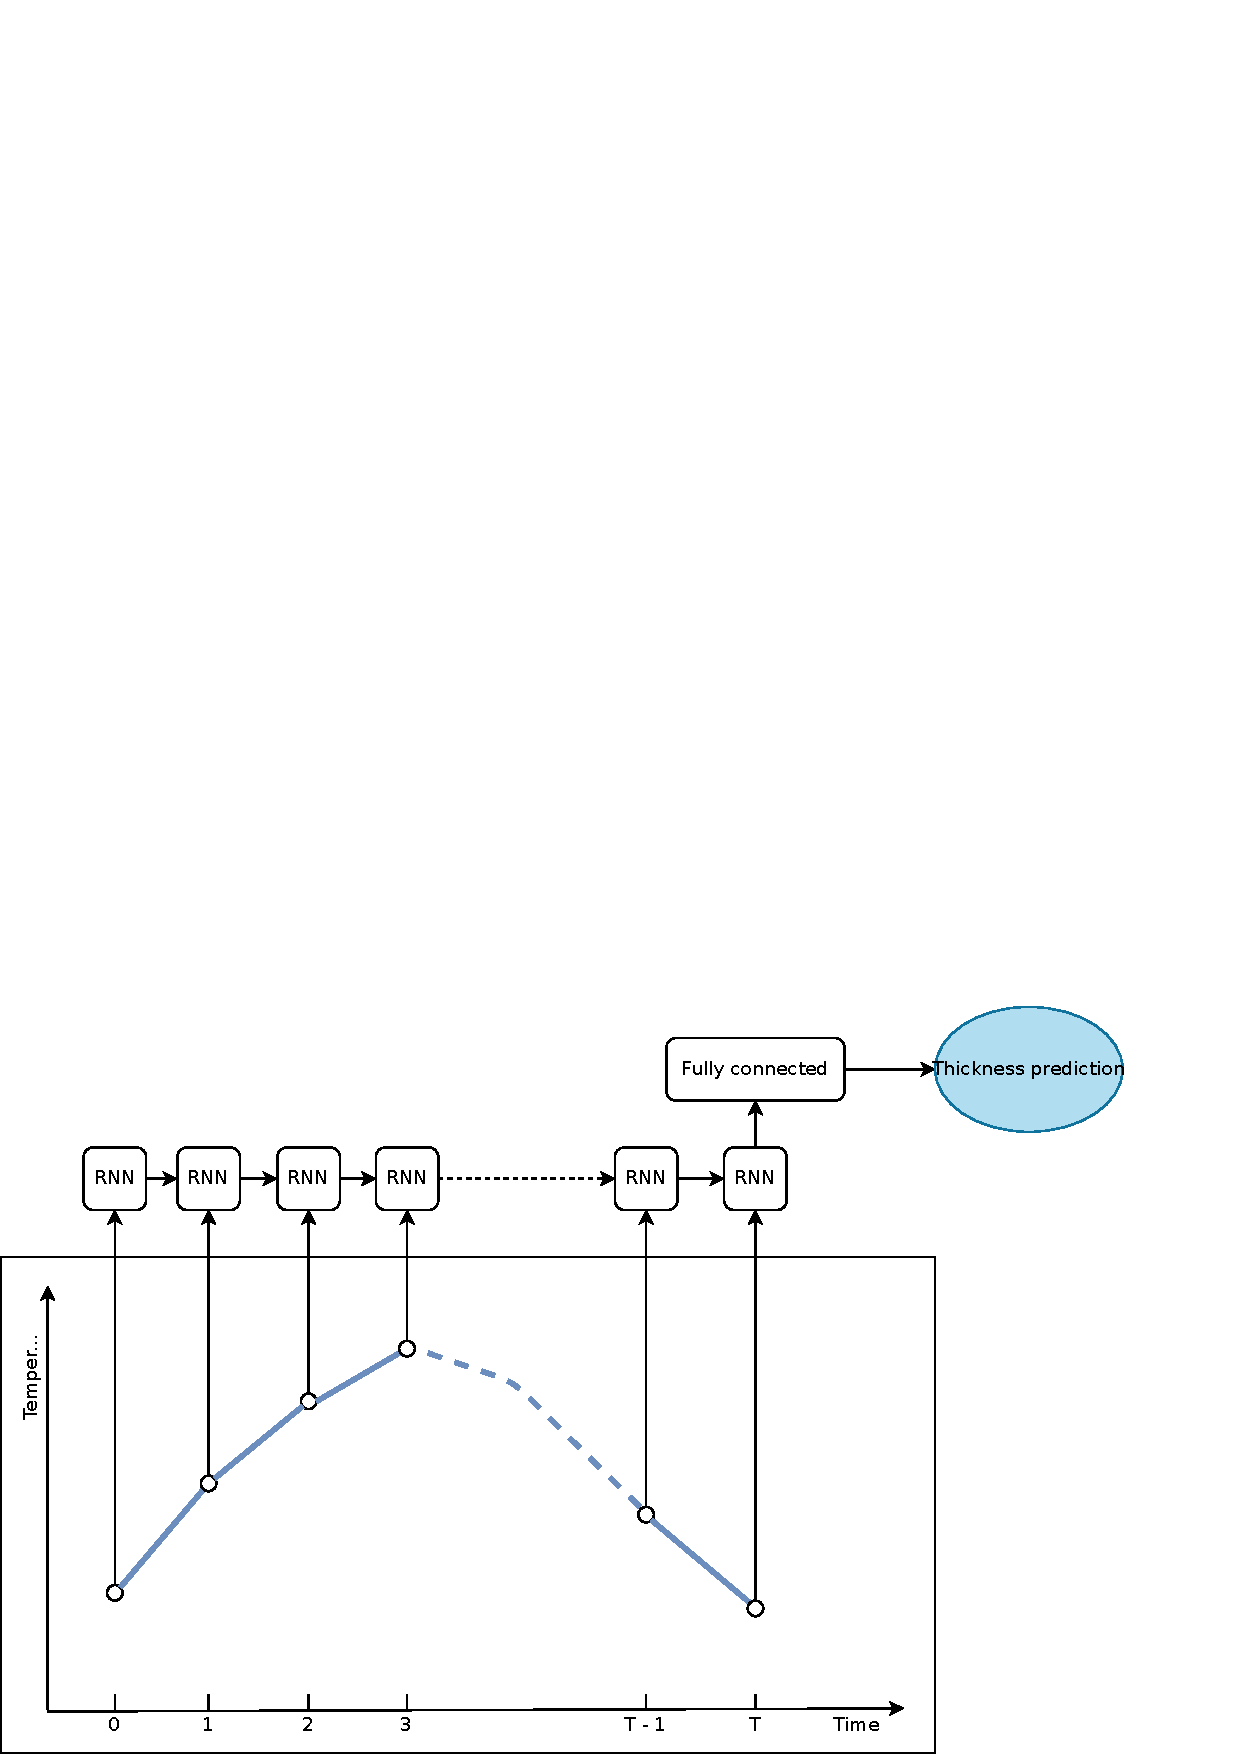
\includegraphics[scale=0.45]{images/chapter_4/rnn_model.png}
\caption{RNN-based model}
\label{fig:rnn_model}
\end{figure}


\subsubsection{Spatial-temporal approach} \label{Spatial-temporal approach}

Compared to the previous approach, the method proposed in this section aims to leverage not only the temporal temperature information, but also the spatial one. Instead of extracting the temperature time series for each critical point of the blow-molded parts we can design an \textit{end-to-end} deep learning architecture able to directly handle the input thermal video. In such a way we should be able to take into consideration not only the surface-temperature evolution of a point but also its position on the spatial dimension. 
% This part should be improved
In this instance, the input dataset
\begin{equation}
    D = \{(X^{i}, Y^{i})\}_{i=1}^{m},
\end{equation}
is a collection of pairs $(X^{i}, Y^{i})$ where $X^{i}$ is the input thermal video with $Y^{i}$ as its corresponding thickness values vector
\begin{equation}
    Y^{i} = [y^{i}_{(x_1, y_1)}, y^{i}_{(x_2, y_2)}, ..., y^{i}_{(x_j, y_j)}, ..., y^{i}_{(x_n, y_n)}].
\end{equation}
The role of the spatial-temporal approach is to approximate the transfer function $\hat{g}$ so that
\begin{equation}
    Y^{i} = \hat{g}(X^{i}, i \in [1, m]) + \epsilon.
\end{equation}
The work presented in this paragraph is largely inspired by the computer vision domain of \textit{Semantic Segmentation}. Semantic image segmentation, or semantic segmentation is the task of clustering the pixels of an image that belong to the same object (or object class). Basically for an input image, semantic segmentation produces a segmentation mask which has the same spatial dimension of the input image where each pixel value correspond to the predicted class. As for other computer vision tasks, state-of-the-art results are obtained through the application of Convolutional Neural Networks (Section \ref{Convolutional Neural Network}).

One popular approach for image segmentation models is to follow an encoder/decoder structure where we “downsample” the spatial resolution of the input, developing lower-resolution feature mappings which are learned to be highly efficient at discriminating between classes, and the “upsample” the feature representations into a full-resolution segmentation map. The encoder-decoder approach, as part of the semantic segmentation domain, was proposed for the first time by \citet{long2015fully} in the Fully Convolutional Network (FCN) architecture and it has been subsequently taken up by other research works \citep{ronneberger2015u,zhao2017pyramid,chen2017rethinking,chen2018encoder,badrinarayanan2017segnet}. The encoder, or contracting path, is, most of the time, a Convolutional Neural Network whose task is to extract features of different spatial resolutions, constituting the so-called “Feature Map”. Compared to the encoder, which reduces the spatial dimension in every layers and increases the channels, the decoder, or expansive path, has the role of restoring the original spatial dimensions by sequentially increasing the spatial dimension while reducing the number of channels. The decoder can be composed of one of multiple decoder block, in the same way the encoder can be more or less deep. Each decoder block computes two different operations: at first it up-sample the feature map using an interpolation method, then it applies a convolutional operation which halves the number of feature channels. Finally, a last convolutional block, sometimes called Segmentation Head, stacked right after the last decoder block produces the segmentation mask.

Instead of predicting a segmentation mask where each pixel belongs to a predefined class, we propose to take advantage of the encoder-decoder architecture to learn reconstructing the thickness of some critical areas of the part. In order to deal with our problem, we have designed an end-to-end pipeline able to provide the critical point values inference given the input video (Figure \ref{fig:proposed_architecture}). 
% The following image will be replaced
\begin{figure}
\centering
\includegraphics[scale=0.45]{images/chapter_4/proposed_architecture.png}
\caption{Proposed architecture (IMAGE WILL BE REPLACED)}
\label{fig:proposed_architecture}
\end{figure}
The proposed pipeline is largely inspired by the encoder-decoder paradigm and in particular to the \textit{Unet} architecture proposed in \citet{ronneberger2015u}. The \textit{Unet} improves the \textit{FCN} architecture by proposing an expansive path which is more or less symmetric to the contracting path that yields a u-shaped architecture. Moreover, the expansive pathway combines the feature and spatial information through a sequence of up-convolutions and concatenations with high-resolution features from the contracting path. By introducing skip connections in the encoder-decoded architecture, fine-grained details can be recovered in the prediction. 
The presented pipeline consists of three main blocks: the spatial encoder, the temporal encoder and the decoder. 

\begin{itemize}
    \item \textit{Spatial Encoder:} The spatial encoder is a CNN which aims to extract the spatial feature map for each frame of the video. The spatial encoder corresponds to the encoder of a traditional encoder-decoder architecture. Compared to the original \textit{Unet} architecture, we replace the original contracting path proposed in the paper with a Residual Network (\ref{Residual Networks}). The ResNet architecture, independently of its depth, it is composed of five main building blocks. Each block sequentially produce lower-resolution feature which will later be used by the decoder to help reconstructing the prediction mask. Given an input thermal video with dimensions $(h, w, c, t)$ where $h$, $w$, $c$ and $t$ are respectively the height of the image, the width, the number of channels and the number of frames of the video sequence. The spatial encoder process each frame $(h, w, c)$ of the input video and it returns a feature maps of size $(h', w', c', t)$ where $h'<<h$, $w'<<w$ and $c'>>c$ and a set of intermediate feature maps.

    \item \textit{Temporal Encoder:} The temporal encoder aims to encode the temporal information of the spatial feature map produced by the spatial encoder. In fact, the spatial encoder encode each frame independently without leveraging any kind of temporal information. In order to encode the temporal information we use a 3D convolutional layers with a kernel size of $(1\times1\times1)$, stacked right after the spatial encoder, which produces a linear projection of the stack of frame-wise feature maps. This projection acts as a dimensional reduction of the temporal dimension. In such a way we are able to produce a new feature map which encode either the spatial and the temporal information. Given the spatial feature map of size $(h', w', c', t)$, the temporal decoder compress the temporal dimension and produces a new \textit{spatial-temporal feature map} with size $(h', w', c', 1)$.  The same convolutional operation, with the same parameters, is applied to compress the temporal information of all the intermediate features maps produced by the spatial encoder.
    
    \item \textit{Decoder:} The decoder projects the discriminative spatial-temporal feature map, to the original input spatial dimension. In the same way as for the \textit{Unet} architecture, intermediate high-resolution features from the encoder path are combined and reused with the upsampled output of each decoder block to help the model reconstructing the prediction mask. The decoder is composed on five decoder blocks and each decoder block applies an upsample operation using the nearest neighbour algorithm followed by two 2D convolutional layers with a kernel size of $3\times 3$, batch normalisation and \textit{ReLu} activation function. A final convolutional layers produce the thickness mask from which the prediction of the critical thickness points are extracted. Given the incoming data of size $(h', w', c', 1)$ the decoder project the encoded pattern to the original spatial dimension producing a 1-channel mask reconstruction $(h, w, 1)$. Given the pixel coordinates of the $n$ critical points, its corresponding thickness prediction can be easily retrieved.
\end{itemize}

Training such an architecture can be a bit more challenging compared to that of the temporal approach because of the number of learnable parameters. Furthermore, we have two main drawbacks:

\begin{itemize}
    \item The size of the training sample is low compared to what is normally used to train this kind of network. For Semantic Segmentation tasks, a dataset of 1000 images is considered small and we hardly would be able to have more than a few hundreds input samples.
    \item The thickness ground-truth map is not known for all the points of the tanks. Semantic Segmentation tasks require, during the training phase of the algorithm, that output mask of the input data is well known. For our problem, the full thickness map of the measured tanks is missing, only a limited number of thickness points are known.
\end{itemize}

The first drawbacks may be potentially handled by applying two different well-known machine learning techniques: \textit{transfer learning} and \textit{data augmentation}. Instead of training a model from scratch, a network with pre-trained parameters may be used as a starting point. Scientific literature suggests that using a pre-trained network would allow to converge faster towards the best solution, especially if the size of the training data is small. Most of the state-of-the-art semantic segmentation approaches make use of pre-trained encoders to start with, while the remaining part of the network is trained from scratch. The use of a pre-trained network is always possible as long the shape of the input data is consistent with the one of the original data used to train the network. 

A second available option to deal with a small dataset would be to make use of the data augmentation technique. Data augmentation in data analysis are techniques used to increase the amount of data by adding slightly modified copies of already existing data or newly created synthetic data from existing data. Popular image augmentation techniques involves geometric transformations such as image flipping, rotation or translation, or colour space transformations. More advanced techniques make use of generative models to create artificial training sample. Regarding our problem, the only augmentation techniques that can be applied are the ones that involves geometric transformation. 
\begin{figure}
\centering
\includegraphics[scale=0.8]{images/chapter_4/data_augmentation.png}
\caption{Image Augmentation}
\label{fig:image_augmentation}
\end{figure}

In fact, since the colour of the image is proportional to the temperature, every augmentation techniques that involves any kind of change in the colour space may completely corrupt the input data.
If the missing of a large volume of input data could be handled with transfer learning and data augmentation, the lack of labelled data in the training dataset may be a little more challenging. In fact, since the full thickness mask of the part is missing, we cannot train the model in classical pixel-wise manner. Traditional semantic segmentation architectures are trained by compute the pixel-wise loss between the ground truth segmentation mask and the reconstruction computed by the network. The computed loss is than back-propagated in the network to adjust the learnable parameters of the architecture. In our particular case, the full thickness ground truth of the part is not known, which means that we cannot compute the pixel-wise loss for all the pixels. It is however still possible to train the network by computing the pixel-wise loss between the mask and the reconstruction only for pixels for which the thickness is known.

\section{Experimental Validation} \label{Experimental Validation}

This section presents the results from a real-world implementation in an industrial case. First, the empirical setting is described as well as the data processing and the training pipeline. Finally we provide the results of this first experimentation.

\subsection{Data collection}

To evaluate the performance of the proposed data-driven model-based quality control, a data acquisition campaign in an industrial environment has been organised. In order to train our models to learn to infer the thickness, given the cooling profile, we need two different types of data: the temperature of the part surface and the thickness measurement of the corresponding part. The Temperature data  has been acquired with an industrial thermal camera OPTRIS PI 640 with a good resolution (640$\times$480), previously calibrated to correctly measure the temperature of the plastic material. Unlike traditional colour images, which are commonly represented using a 3-channel matrix (\textit{RGB}) with 256 different integer values, thermal images collected through the OPTRIS 640 PI are 1-channel matrices where each pixel takes a continuous value corresponding to a temperature in degrees Celsius. Unlike other temperature measuring instruments, the thermal camera has the advantage to evaluate, in a single shot, the temperature of the whole visible surface. Several consecutive shots of the same part make it possible to follow the evolution of the temperature over time (Figure \ref{fig:thermal_video}). 

Before moving forward in the description of the empirical setting, a clarification is needed. Previously, we said that thermal images are 1-channel matrix where each pixel take a continuous value corresponding to a temperature in degree Celsius . Because computers interprets as images only matrix (or 3D tensors) composed of unsigned integers, composed of values ranging from 0 to 255, to display a thermal image is necessary to map the continuous temperatures values to the 0-255 range. In others words, a \textit{colormap} needs to be applied to the raw images in order to display it. In Figure \ref{fig:thermal_video}, as well as for others images of the current chapter, thermal frames are 

\begin{figure}
\centering
\includegraphics[scale=0.55]{images/chapter_4/Thermal_video.png}
\caption{Thermal video $X_i$}
\label{fig:thermal_video}
\end{figure}

Of course, measuring the temperature of the entire surface of the part would require several cameras. As part of the presented experiment, we decided to limit the temperature acquisition to half of the whole surface. The thickness measurement has been carried out on critical points through the use of an ultrasonic measurement instrument routinely used for sampling control. The thickness values of the part selected for our experimentation have typical values ranging between 3 and 10 millimetres. In order to gather comparable data, the image acquisition of each part produced needs to be synchronised with the blowing process in order to synchronise the  acquisition of images on the same relative time. Repeatable mechanical movements of the machine have been used to “trigger” data acquisition. The trigger starts a one minute countdown after which the acquisition of thermal images will begin. This time is mandatory to give the machine the time to unload the part and the machine operator time to place the part in the measuring area. In the experimental context described here, the part is positioned on a table and, at the end of the one minute countdown, the thermal camera starts collecting images. For our experimental measurement campaign, we collected thermal videos on 50 different parts. For each part we recorded 120 consecutive thermal images equally spaced  with a one second interval between one image and the next, for a total of two minutes of data acquisition. For each thermal video, and therefore for each part, we measured 20 critical thickness points evenly distributed on the tank surface (see Figure \ref{fig:critical_points}). 

\begin{figure}
\centering
\includegraphics[scale=1]{images/chapter_4/critical_points.jpg}
\caption{Critical points distribution on the tank surface}
\label{fig:critical_points}
\end{figure}


\subsection{Data processing}

Once the data is collected, some processing operations are needed to prepare data for training. In particular, we need to associate the 20  measured critical thicknesses of the part to their corresponding pixel coordinates on the thermal video. This was done manually, each measured point of the part is identified on the thermal image as a $(x_j, y_j)$ pixel coordinate. Hopefully, since the position of the part does not change during the image acquisition, it is enough to find the pixel coordinates for the first frame. 

Although we can assume that the part does not move during the acquisition, each part is positioned identically with respect to the field of view of the thermal camera. The  $(x_j, y_j)$ coordinates on different thermal videos may therefore refer to different surface areas of the part. In order to align pixel coordinates along parts, a transformation is applied, to each frame, to project the part onto a reference. Before describing the transformation in more detail, we present the \textit{Pinhole camera model}. 

\paragraph{The Pinhole camera model}
The pinhole camera model describes the mathematical relationship between the coordinates of a point in a three-dimensional space and its projection onto a two-dimensional pixel coordinate system. This mathematical relationship depends on the extrinsic and intrinsic parameters of the camera. The extrinsic parameters refer to the rotation matrix and translation vector of the camera coordinate system with regard to the world coordinate system.
Given a point $(x, y, z, 1)^{T}$ in the world coordinate system, we can form its pixel coordinates $(u, v, 1)^{T}$ as follows:
\begin{equation*}
    s\begin{bmatrix} u\\ v\\ 1 \end{bmatrix} = \begin{bmatrix}
        f_x & 0   & c_x\\ 
        0   & f_y & c_y \\ 
        0   & 0   & 1 
        \end{bmatrix}
        \begin{bmatrix}
        r_{11}& r_{12} & r_{13} & t_{x} \\ 
        r_{21}& r_{22} & r_{23} & t_{y} \\
        r_{31}& r_{32} & r_{33} & t_{z}
        \end{bmatrix}
        \begin{bmatrix} x\\ y\\ z \\ 1 \end{bmatrix}
        \enspace,
\end{equation*}
That is:
\begin{equation*}
    s\begin{bmatrix} u\\ v\\ 1 \end{bmatrix} = K[R|T]
    \begin{bmatrix} x\\ y\\ z \\ 1 \end{bmatrix}
        \enspace,
\end{equation*}

where:
\begin{itemize}
    \item $K$ is the 3 $\times$ 3 intrinsic camera matrix.
    \item $f$ is the focal length.
    \item $(u_0,v_0)$ are the coordinates of the principal point at the center of the image plane.
    \item $R$ is the 3 $\times$ 3 rotation matrix.
    \item $T$ is the translation vector.
    
\end{itemize}

Given this  mathematical description, a homography $H$ can be defined as a transformation matrix that maps points from one plane to another. It can be derived by the equation REF:

\begin{equation*}
    \begin{bmatrix} u\\ v\\ 1 \end{bmatrix} = \begin{bmatrix}
        f_x & 0   & c_x\\ 
        0   & f_y & c_y \\ 
        0   & 0   & 1 
        \end{bmatrix}
        \begin{bmatrix}
        r_{11}& r_{12} & r_{13} & t_{x} \\ 
        r_{21}& r_{22} & r_{23} & t_{y} \\
        r_{31}& r_{32} & r_{33} & t_{z}
        \end{bmatrix}
        \begin{bmatrix} u'\\ v'\\ 0 \\ 1 \end{bmatrix}
\end{equation*}

\begin{equation*}
    \begin{bmatrix} u\\ v\\ 1 \end{bmatrix} = \begin{bmatrix}
        f_x & 0   & c_x\\ 
        0   & f_y & c_y \\ 
        0   & 0   & 1 
        \end{bmatrix}
        \begin{bmatrix}
        r_{11}& r_{12} & t_{x} \\ 
        r_{21}& r_{22} & t_{y} \\
        r_{31}& r_{32} & t_{z}
        \end{bmatrix}
        \begin{bmatrix} u'\\ v'\\ 1 \end{bmatrix}
\end{equation*}

\begin{equation*}
    \begin{bmatrix} u\\ v\\ 1 \end{bmatrix} = 
        \begin{bmatrix}
        h_{11}& h_{12} & h_{13} \\ 
        h_{21}& h_{22} & h_{23} \\
        h_{31}& h_{32} & h_{33}
        \end{bmatrix}
        \begin{bmatrix} u'\\ v'\\ 1 \end{bmatrix}
\end{equation*}

\begin{equation} \label{projection}
P=HP'
\end{equation}

where:

\begin{itemize}
    \item $P$ and $P'$ are two points on different planes.
    \item $H$ is a 3 $\times$ 3 matrix composed by intrinsic and extrinsic parameters that relate the two planes together.
\end{itemize}


The mathematical framework presented above can be applied to project all the thermal frames composing the 50 thermal video collected over a reference image. By estimating the homography between the two planes, that of the reference image and that of the image to be projected, each point $P$ of the input image could be projected to the reference image. 

The first frame of each thermal video sequence is used to estimate the homography matrix, through the use of the ORB (Oriented FAST and Rotated BRIEF) algorithm \citep{rublee2011orb}. In a nutshell, ORB is a feature matching algorithm that allows to automatically find some key-points in an image. The ORB algorithm takes as inputs two images, a reference and the one we want to project on this reference, and features that can be matched in the two images are used to estimate the homography matrix. Once the homography is computed, it is applied to map all the pixels of the second image to the pixel of the reference image. The same transformation can then be applied to all the frames in the video sequence, provided that both the camera and the tank are motionless. 
%
Then, depending on the used method, between the functional, temporal and the spatial-temporal, extra processing is needed to prepare data for training.

\subsubsection{Functional approach}
The Functional approach makes use of the temperature time series extracted from the thermal video sequences to infer the corresponding thickness. Given the coordinates $(x_j, y_j)$ of the 20 critical thickness values, it is simple to retrieve the temperature time series by simply collecting the temperature of the coordinate for each sequential frame of the thermal video. By extracting all temperature time series for each critical point of the 50 parts considered, we can build a new time series dataset composed of 1000 (50 x 20) time series and the corresponding thickness values. The time series are then approximated by their parametric expansion. As explained in Section \ref{Functional approach}, three different parametric functions have been identified as good candidates for approximating the pixel-wise temperature surface decay. In order to identify the parametric expansion that best fits the input time series, each expansion was applied to the time-series of the training set. The root mean square error (RMSE) of the overall reconstruction is used to select the best expansion. 

Table \ref{tab:curve_fitting_error} shows the average  RMSE reconstruction for the three parametric expansions considered. The polynomial expansion minimises the reconstruction error and is thus used to summarise the raw time series. 
For each time series, the three parameters defining the second-order polynomial approximation constitute the predictor of the machine learning model.

\begin{table}
\centering
\begin{tabular}{|l|l|}
\hline
Parametric function    & RMSE (train) \\ \hline
Power Law              & 0.29         \\ \hline
Logarithmic            & 0.27         \\ \hline
Polynomial (2° degree) & 0.03         \\ \hline
\end{tabular}
\caption{Curve fitting reconstruction error}
\label{tab:curve_fitting_error}
\end{table}


\subsubsection{Temporal approach}

As for the functional approach, the Temporal approach makes use of the temperature time series extracted from the thermal video sequences to infer the corresponding thickness. Given the coordinates $(x_j, y_j)$ of the 20 critical thickness values, it is simple to retrieve the temperature time series by simply collecting the temperature of the coordinate for each sequential frame of the thermal video. Unlike the previous approach, no extra data processing is required because the raw time series constitute the input data of the RNN model. 

\subsubsection{Spatial-Temporal approach}
Compared to the temporal approach, the spatial-temporal approach also leverages the spatial information contained in the video. It does not require to rearrange the input thermal video in another data structure, but some processing operations are still needed to allow the usage of a pre-trained spatial encoder. In order to be consistent with the data of the \textit{ImageNet} dataset \citep{deng2009imagenet} that was used  to pre-train the network, each thermal frame is converted to a 3-channel RGB image. The maximum and minimum temperatures among all frames are retrieved and the same colormap is applied on all thermal frames of each video sequence. The colormap is the one applied to visualise the thermal frames in the current Chapter. All values are then rescaled in $[0, 1]$ and then normalized using the default mean and standard deviation value of the \textit{ImageNet} dataset.

\subsection{Training}

In this section our training pipeline is presented. For each approach, the data was divided into three sets: the training set (data from 38 parts), the validation set (data from 8 parts) and the test set (data from 5 parts). The training is used to train the model, the validation set is used to evaluate the performance of our methods for each combination of model hyper-parameters and finally, the test set is used to evaluate the ability of the model to generalise the results obtained on new data. For each proposed approach, a Bayesian optimization of hyper-parameters with the \textit{Tree-structured Parzen Estimator} (TPE) \citep{bergstra2011algorithms} algorithm was used to select the hyper-parameters that minimise the \textit{Mean Squared Error} (MSE) on the validation set. The TPE sequentially selects the new hyper-parameters to be tested, thus avoiding an exhaustive grid search, which is quickly too demanding in terms of computing resources.

\subsubsection{Functional approach}

As explained previously, a second-degree polynomial is fitted over the time series to compress the input data in a few features corresponding to the coefficients of the polynomial expansion of the thermal signal. Three machine learning algorithms were compared to model the relationship between the polynomial coefficients and the corresponding thickness values: \textit{Lasso} (linear) regression, \textit{random forest} and \textit{Support Vector Machine} (linear or kernelized) regression. For all models,  hyper-parameters have been optimised by the TPE algorithm (See Section \ref{TPE approach}). 
%Every combination of hyper-parameter values is tested to find the one that minimize the cost function.
%
The exhaustive list of model hyper-parameters and their search space is summarized in Table \ref{tab:functional_search_space}.

\begin{table}
\centering
\label{tab:functional_search_space}
\caption{Hyper-parameter search space for the functional models}
\begin{tabular}{lll} 
\toprule
\textbf{Model}                            & \textbf{Hyper-parameter} & \textbf{Search space}                          \\ 
\midrule
Lasso                                     & $\lambda$                & LogSpace($10^{-5}$, 1)                          \\ 
\midrule
SVM  & Kernel                   & \{Linear, Polynomial, RBF\}  \\ 
\cline{2-3}
                                          & $C$                        & LogSpace($10^{-6}$, 1)                          \\ 
\midrule
\multirow{3}{*}{Random Forest}  & Number of estimators     & {[}50, 51, 52, ..., 500]                       \\ 
\cline{2-3}
                                          & Maximum tree depth       & {[}4, 5, 6, ..., 50]                           \\ 
\cline{2-3}
                                          & Minimum samples leaf     & {[}1, 2, 3, ..., 60]                           \\
\bottomrule
\end{tabular}
\end{table}


\iffalse
\begin{table}
\centering
\begin{tabular}{|l|l|p{5cm}|} 
\hline
\multicolumn{3}{|c|}{Functional approach: model hyper-parameters search space}                                                 \\ 
\hline
\textbf{Model}                            & \textbf{Hyper-parameter} & \textbf{Search space}                          \\ 
\hline
Lasso                                     & $\lambda$                & LogSpace($10^{-5}$, 1)                          \\ 
\hline
\multirow{2}{*}{Support Vector Regressor} & Kernel                   & {[}Linear, Polynomial, Radial basis function]  \\ 
\cline{2-3}
                                          & $C$                        & LogSpace($10^{-6}$, 1)                          \\ 
\hline
\multirow{3}{*}{Random Forest Regressor}  & Number of estimators     & {[}50, 51, 52, ..., 500]                       \\ 
\cline{2-3}
                                          & Maximum tree depth       & {[}4, 5, 6, ..., 50]                           \\ 
\cline{2-3}
                                          & Minimum samples leaf     & {[}1, 2, 3, ..., 60]                           \\
\hline
\end{tabular}

\caption{Functional model search space}
\label{tab:functional_search_space}
\end{table}
\fi

\subsubsection{Temporal approach}
We compared the performance of three RNN-based models: a vanilla RNN, an LSTM and finally a GRU network. The number of hidden units of each computational cell, as well as the number of stacked layers are hyper-parameters that are optimised. A comprehensive summary of the search space for the hyper-parameters is available in Table \ref{tab:rnn_search_space}. 

\begin{table}
    \centering
    \begin{tabular}{|p{3cm}|p{4cm}| }
    \hline
    \multicolumn{2}{|c|}{Temporal approach: model hyper-parameters search space} \\
    \hline
    RNN Cell type & [RNN, LSTM, GRU] \\
    \hline
    N° hidden unit & [8, 16, 32] \\
    \hline
    N° stacked layers & [1, 2] \\
    \hline
    \end{tabular}
    \caption{Temporal approach: model hyper-parameters search space}
    \label{tab:rnn_search_space}
\end{table}
Each model has been trained to minimise the mean squared error metric using the  \textit{Adam} optimiser~\citep{kingma2014adam} with $\beta_{1} = 0.9$, $\beta_{2} = 0.98$ and $\epsilon = 10^{-9}$ and a learning rate sampled by the TPE algorithm on a logarithmic scale,  from $10^{-7}$ to $10^{-2}$. 

\subsubsection{Spatial-Temporal approach}
As for the previous approach, we compared different model configurations on two pre-trained networks: a ResNet18 (18 layers) and a ResNet34 (34 layers). Deeper architectures exist, but we made the choice to limit the search space to the two smaller ResNet architectures because of the limited number of samples in our training set. In fact, deeper architectures allow to extract more complex data representations at the expense of a greater number of parameters and increased computation time. We claim that ResNet18 and ResNet34 are powerful enough to produce a discriminant representation. Another hyper-parameters of the presented architecture is the number of encoder, and decoder, blocks. As stated in section \ref{Residual Networks}, all ResNet architectures, independently on their depths, have 5 main convolutional blocks. Actually, it is possible to slightly change the architecture in order to stop the encoding computation before the last block. This allows to reduce the complexity of the architecture and thus prevent possible over-fitting problems. For instance, we could take into account only the first 3 convolutional building blocks of the ResNet in such a way that the output of the third convolutional building block would be the spatial feature map and the output of the first and second blocks would be the intermediate encoded features. Since the encoder and decoder are symmetrical, reducing the number of encoder blocks also implies a reduction in the number of decoder blocks.

\begin{table}[h!]
    \centering
    \begin{tabular}{|p{3cm}|p{4cm}| }
    \hline
    \multicolumn{2}{|c|}{Spatial-Temporal approach: model hyper-parameters search space} \\
    \hline
    Encoder & [ResNet18, ResNet34] \\
    \hline
    N° of blocks  & [3, 4, 5] \\
    \hline
    \end{tabular}
    \caption{Spatial-Temporal approach: model hyper-parameters search space}
    \label{tab:spatial_temporal_search_space}
\end{table}

% Talk about different loss function
As for the Temporal approach, each model configuration has been trained to minimise the MSE metric using \textit{Adam} optimiser with $\beta_{1} = 0.9$, $\beta_{2} = 0.98$ and $\epsilon = 10^{-9}$ and a learning rate sampled by the TPE algorithm on a logarithmic scale from $10^{-10}$ to $10^{-2}$. 

\subsection{Results}

In this section the results obtained with the three approaches are presented and compared. Performances are measured using the Root Mean Squared Error (RMSE), which has the benefit of penalising large errors and whose value is easy to interpret because it has the same unit as the dependent variable. This means that all the scores presented below represent the average thickness reconstruction error in millimetres.

For the functional approach, random forest performs better in both fit on the training set and generalization on the test set (Table \ref{tab:functional_model_results}).
%
\begin{table}[h!]
    \centering
    \begin{tabular}{|l|p{2.8cm}|p{2.8cm}|p{2.8cm}|}
    \hline
    \multicolumn{4}{|c|}{Functional approach: best model} \\
    \hline
    Model & RMSE train  & RMSE validation  & RMSE test  \\
    \hline
    Lasso & \textbf{0.95} & \textbf{0.91} & \textbf{0.89} \\
    \hline
    Support Vector Regressor & \textbf{0.80} & \textbf{0.73} & \textbf{0.76} \\
    \hline
    Random Forest Regressor & \textbf{0.19} & \textbf{0.54} & \textbf{0.48} \\
    \hline
    \end{tabular}
    \caption{Functional model results}
    \label{tab:functional_model_results}
\end{table}
%
The error is about 0.5 mm, which is not totally satisfactory from an industrial point of view. However, this first experiment allowed us to demonstrate that there is a relationship between the temperature evolution of a zone of the part and the corresponding thickness, as assumed in  Section \ref{Motivation}.

\begin{figure}
\centering
\includegraphics[scale=0.48]{images/chapter_4/temporal_scatter.png}
\caption{Prediction \textit{versus} ground truth scatter plots in train (left) and test (right) for the functional approach based on random forest regression}
\label{fig:gt_prediction_functional}
\end{figure}

Figure \ref{fig:gt_prediction_functional} shows the scatter plots of the predicted thickness and ground-truth thickness for the training set and the test set. The plots confirm the ability of the modef to distinguish between large and small thicknesses. Moreover, they show that the model is more accurate for thin points  (close to 3 mm). This observation is encouraging because the thinnest points are also the most critical to ensure that the part meets the customer's specifications.

Among all temporal trained model, the configuration that minimises the validation error is a GRU model with 8 hidden units per cell and one layer. The results obtained are summarised in Table \ref{tab:temporal_model_results}.
%
\begin{table}
    \centering
    \begin{tabular}{|p{3.2cm}|p{3.2cm}|p{3.2cm}|p{3.2cm}|}
    \hline
    \multicolumn{4}{|c|}{Temporal method: best model} \\
    \hline
    Model & RMSE train  & RMSE validation  & RMSE test  \\
    \hline
    GRU & \textbf{0.54} & \textbf{0.56} & \textbf{0.55} \\
    \hline
    \end{tabular}
    \caption{Temporal model results}
    \label{tab:temporal_model_results}
\end{table}
%
These results are similar to those obtained with random forest, but random forest has a slightly lower error than GRU. Moreover, the computation time needed to train the random forest is significantly lower and it does not require dedicated hardware (GPU). The functional approach therefore seems preferable in all respects. This is confirmed in Figure~\ref{fig:gt_prediction_temporal}, where the functional approach outperforms the temporal approach over all thickness ranges.
\begin{figure}
\centering
\includegraphics[scale=0.48]{images/chapter_4/gt_temporal.eps}
\caption{Prediction \textit{versus} ground truth scatter plots in train (left) and test (right) for the temporal approach based on GRU}
\label{fig:gt_prediction_temporal}
\end{figure}

The third approach (Table \ref{tab:spatial_temporal_model_results}) completely outperforms the previous ones. The best results are obtained using a pre-trained ResNet34 encoder with 5 encoder-decoder blocks, which achieves an RMSE of 0.16 mm on the test set, which is about one-third of the error of the previous approaches. An error of the order of 0.2mm is considered extremely interesting in our industrial context. 
\begin{table}
    \centering
    \begin{tabular}{|p{3.5cm}|p{3.2cm}|p{3.2cm}|p{2.8cm}|}
    \hline
    \multicolumn{4}{|c|}{Spatial-Temporal method: best model} \\
    \hline
    Model & RMSE train  & RMSE validation  & RMSE test  \\
    \hline
    ResNet34-5 blocks) & \textbf{0.14} & \textbf{0.18} & \textbf{0.16} \\
    \hline
    \end{tabular}
    \caption{Spatial-Temporal model results}
    \label{tab:spatial_temporal_model_results}
\end{table}
Figure~\ref{fig:gt_prediction_spatial_temporal} shows that the greatest benefits over the functional approach are at higher thicknesses, but the improvement is already visible at only 4 mm.

\begin{figure}
\centering
\includegraphics[scale=0.48]{images/chapter_4/gt_spatial_temporal.eps}
\caption{Prediction \textit{versus} ground truth scatter plots in train (left) and test (right) for the spatial-temporal approach based on ResNet34}
\label{fig:gt_prediction_spatial_temporal}
\end{figure}

\subsection{Model performance on unseen data point}

% This section should be improved

The results presented in the previous section highlighted the ability of the spatial-temporal model to correctly estimate thicknesses at the critical points of the part.  It is questionable whether the model is able to generalise what it learned for a limited set of critical points to the entire surface of the part. The Spatial-Temporal architecture has been designed to provide, as output, the thickness reconstruction for all the pixels belonging to the tank surface. An example of reconstruction of the thickness mask, produced by the Spatial-temporal architecture, is visible in Figure \ref{fig:thickness_mask_reconstruction}. This figure represents the thickness reconstruction of a random sample belonging to the test set. Unlike the previous images, this time the intensity of the colour is not related to the temperature of the tank, but represents its thickness.
The Figure highlights the ability of the model to produce a thickness reconstruction for all the points belonging to the part surface. However, it struggles to reconstruct some areas, especially those close to the edge of the tank. The ability to predict sensible thicknesses outside the critical points is questionable.

\begin{figure}
\centering
\includegraphics[scale=0.90]{images/chapter_4/mask_reconstruction.png}
\caption{Thickness mask reconstruction example}
\label{fig:thickness_mask_reconstruction}
\end{figure}

In order to test this ability, we modified the validation strategy. Since the entire thickness mask is not available, we used only a subset of the 20 critical thickness values to train the model, reserving the others to compute the prediction error. %Unfortunately, we cannot remove too many points because, in that case, we would deprive the model of too much information.
We removed 4 out of 20 critical points and trained the model on the remaining points. The 4 points removed are then  used to evaluate the ability of the model to predict the thickness outside the critical points. This operation was repeated 20 times by randomly selecting the 4 removed points. In this way, it is possible to evaluate the results on a larger set, composed of $4\times20$ samples.
For each iteration of the algorithm, the same architecture and the same hyper-parameters are used. Results are presented in Figure \ref{fig:gt_prediction_unseen} that shows a positive correlation between ground truth and prediction. 
%
% Should I add a pseudo-code to explain the validation strategy ? 

\begin{figure}
\centering
\includegraphics[scale=0.90]{images/chapter_4/unseen_point_scatter.png}
\caption{Prediction \textit{versus} ground truth scatter plots for the spatial-temporal approach based on ResNet34 on points not seen in training}
\label{fig:gt_prediction_unseen}
\end{figure}
%
However, the prediction of the thickness of unseen points is nowhere near as good as the prediction on unseen parts, and our approach does not meet the industrial requirements in this respect: our model is not reliable when it comes to predicting the thickness of the entire part. In Chapter \ref{Contributions and perspectives} we will present some of the research perspectives we are working on to improve the ability of the model to correctly predict the thickness of the full visible surface. 

\section{Conclusion}

Traditional quality control methods for measuring blow-molded part thickness involves time-consuming operations that cannot be applied online for a 100\% quality inspection. This chapter proposes a new data-driven approach for measuring in real-time the part thickness by leveraging the surface-temperature decay over time. Three different pipelines have been designed to model the relationship between the cooling behavior of a part area, captured through the use of a thermal camera, and the corresponding thickness. The procedure was validated in a real-world manufacturing setting. These results have shown the ability of our method to provide accurate results in predicting thickness values of a set of critical points. Among the three methods presented above, the spatial-temporal approach is the one that achieve the best performance in reconstructing the thickness values of the test set data. 

Future research works would try to generalize what is learned for a limited number of thickness points, in order to potentially reconstruct the full thickness cartography of the whole visible part surface. In Chapter \ref{Contributions and perspectives} we will provide more details about the research perspectives related to this topic. 

\subsection{Scientific Contribution (TO BE COMPLETED)}

This chapter proposes, in our opinion, two mains scientific contributions. At first we have proposed a general framework to improve the control quality of manufactured parts. In particular, we propose to improve the quality control of the manufactured parts by introducing TO BE FINISHED  

Secondly, an application of the current approach in the framework of this thesis project is presented. We have proposed a new approach to infer the thickness of a blow-molded part using a data-driven approach. Three different methods have been proposed. We claims that the same approach could be applied every time that a production process involves TO BE FINISHED

\subsection{Industrial Contribution (TO BE COMPLETED)}

From the industrial point of view, this chapter introduce a new idea of quality control. The traditional Acceptance Sampling approach, used in the industrial context studied, may be enhanced by introducing data-driven model quality control. This approach, which has been proven to be interesting for the task of predicting the thickness of the parts, may be extended to others quality characteristics. Moreover, this approach could also be extended to others process such us the \textit{Post-Cooling}, the \textit{Finishing} or the \textit{Assembly}. By adding extra sensors, or camera, or simply by leveraging the process data collected in the PLC of the machines, it could be possible to provide a quality status to the part without any time-consuming or destructive measurement. 

As regarding the thickness prediction, results are considered accurate enough to move towards the industrialization of the proposed system. In order to industrialize the proposed system, we should be able to take into account extra information such us the temperature of the environment where the machine is located, as well as the temperature of the molds. In fact, the surface temperature of the blow-molded part depends on the ability of the molds to absorb the heat. If the heat absorption capacity changes, as a result of the change in temperature of the molds coolant, the tank surface temperature will be different and the data-driven model accuracy would drop. In the same way, the plant temperature may influence the cooling behavior of the blow-molded part   




